% superlight clients
% sidechains
\section{Our Contributions}
\subsection{Superblocks}

We create a decentralized blockchain client or verifier which, having only
\emph{genesis}, connects to multiple provers, at least one of which is honest,
is able to ascertain the confirmation of a transaction. Using its full local
chain, each prover generates a succinct proof and sends it to the verifier.
Adversarial provers can send anything in the place of a proof. By comparing the
proofs in terms of the amount of proof-of-work they encode, the verifier deduces
which blockchain contains the most proof-of-work without receiving and
validating every block header. The proofs the provers send are only generated
once and do not require multiple interrogation questions from the verifier. As
such, these proofs are non-interactive and we call them \emph{Non-Interactive
Proofs of Proof-of-Work} (NIPoPoWs).

To create such succinct representations of work, we look at the distribution of
block hashes in the chain. Every valid block $B$ satisfies the proof-of-work
equation $H(B) \leq T$ where $T$ is the mining target, but some blocks satisfy
it better than others. Some blocks so happen to have a hash with value
\emph{much} lower than $T$, even though this is not required for validity and is
not intentional. For example, some blocks will satisfy $H(B) \leq \frac{T}{2}$.
Concretely, because the hash function is uniformly distributed, in expectation
\emph{half} the blocks will satisfy $H(B) \leq \frac{T}{2}$, a \emph{quarter} of
them will satisfy $H(B) \leq \frac{T}{4}$, an \emph{eighth} will satisfy $H(B)
\leq \frac{T}{8}$, and in general only a $\frac{1}{2^\mu}$ fraction of blocks
will satisfy $H(B) \leq \frac{T}{2^\mu}$. If a block satisfies this inequality
for some $\mu \in \mathbb{N}$, we say that it is of \emph{level} $\mu$ and call
it a $\mu$-superblock (and note that a $\mu$-superblock for $\mu > 0$ is also
a $(\mu - 1)$-superblock). The probability of a valid block $B$ being a
$\mu$-superblock is:

\[
\Pr[H(B) \leq \frac{T}{2^\mu}|H(B) \leq T] = \frac{1}{2^\mu}
\]

Under this light, the blockchain looks as illustrated in
Figure~\ref{fig.superblocks}. Of course, because block hashes behave randomly,
this image will be probabilistic and blocks may not be precisely distributed as
expected.

\begin{figure}[ht]
    \caption{Superblocks distributed within a blockchain.
    Higher levels have achieved a higher difficulty during
    mining.}
    \centering
    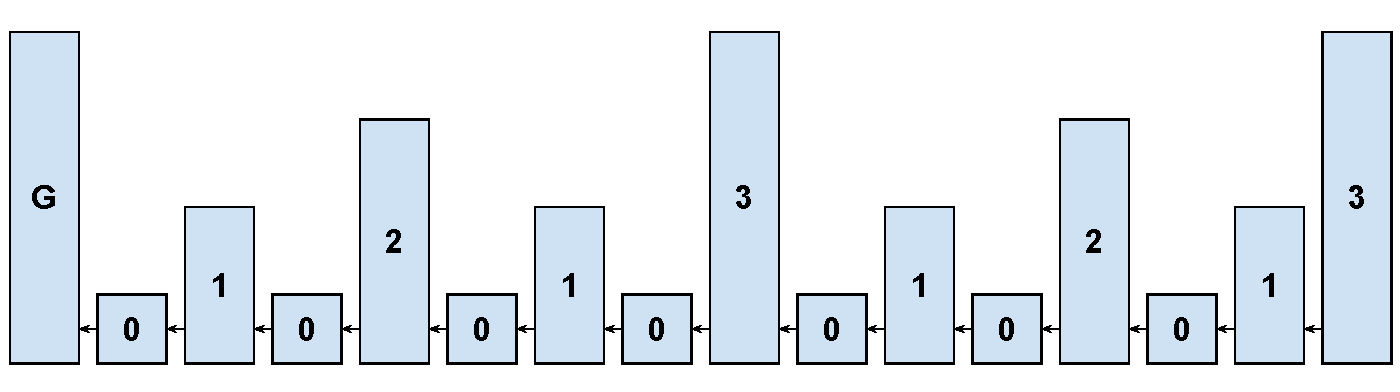
\includegraphics[width=0.7\columnwidth,keepaspectratio]{chapters/introduction/figures/superblocks.pdf}
    \label{fig.superblocks}
\end{figure}

When a chain $\chain$ is mined, there will therefore exist a \emph{subchain} of
it, consisting only of blocks of level $\mu$, which is going to be only
$\frac{|\chain|}{2^\mu}$ blocks long. The core idea of the construction is this:
Instead of sending the full chain, the prover chooses a level $\mu$ and sends
this as a \emph{representative of the underlying work}. Presenting a block of
level $\mu$ captures the fact that work of about $2^\mu$ has happened around it
without presenting that work itself. As such, a superblock is a way for the
prover to \emph{sample} the blockchain in a way that can convince the verifier:
When the verifier receives $m$ blocks of level $\mu$, it can deduce that
approximately $m 2^\mu$ regular blocks must exist around those superblocks.
Constructions based on this simple idea instantiate NIPoPoWs by leveraging
superblocks and we call them \emph{superblock NIPoPoWs}.

A simplified description of our protocol then works as follows. Initially, some value
$m$ is fixed, representing the number of blocks that the verifier wishes to
receive to feel safe. This $m$ is a constant parameter. The honest prover then
chooses the highest level $\mu$ which has at least $m$ blocks at that level.
Choosing any level above $\mu$ would not satisfy the verifier, as fewer than $m$
blocks would be transmitted. Choosing any level below $m$ would be wasteful, as
more blocks would have to be transmitted. This prover choice is illustrated in
Figure~\ref{fig.level-threshold}. Suppose that the verifier receives two
proofs from two provers, one of which is honest while the other adversarial, and
wishes to compare them. The verifier first checks that all the blocks it has
received really are $\mu$-superblocks by verifying the proof-of-work equation
parameterized by $\mu$ is satisfied, and that each proof it has received has at
least $m$ blocks. Then, just as an SPV verifier would compare the length of two
full chains, the NIPoPoW verifier now simply \emph{counts} the number of blocks
it has received from the two provers and announces that the one with the most
blocks is the winner. If the verifier receives the proofs $\pi_1$ and $\pi_2$,
then the decision is simply the result of the comparison $|\pi_1| > |\pi_2|$.

\begin{figure}[ht]
    \caption{A superblock NIPoPoW prover chooses the threshold (dashed line)
    corresponding to level $\mu = 2$ for the verifier requirement $m = 4$.}
    \centering
    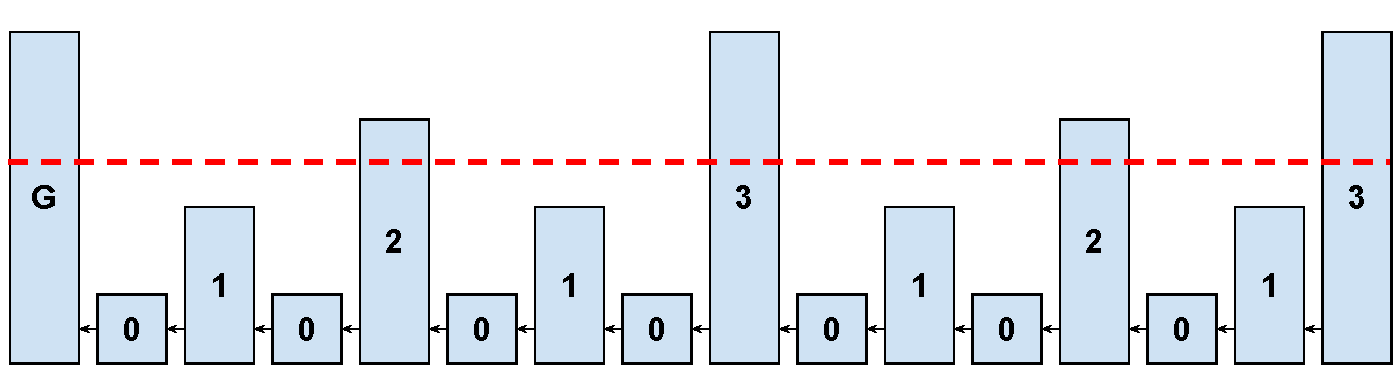
\includegraphics[width=0.7\columnwidth,keepaspectratio]{chapters/introduction/figures/level-threshold.pdf}
    \label{fig.level-threshold}
\end{figure}

The crucial point in terms of security is that an adversary cannot fake this
set of superblocks without actually putting in the work. An adversary that
produces a $\mu$-superblock will also in expectation generate some $2^\mu$
regular blocks in the process (even though the adversary may of course choose
to discard these). Because the adversary has minority mining power, an adversary
cannot create a longer sequence of $\mu$-superblocks faster than the honest
parties create one, for the same reason that an adversary cannot create a longer
regular blockchain faster than the honest parties create one.

Let us count how many different levels $\mu$ there are in a chain. If the chain
has length $|\chain|$, then going up to level $1$ cuts the chain in half, and we
expect to see only $\frac{|\chain|}{2}$ superblocks of level $1$. Moreover, this
continues with subsequent increases in level, until at level $\mu =
\log|\chain|$ we expect to find only $\frac{|\chain|}{2^\mu} = 1$ block. As soon
as we get to level $\log|\chain| + 1$, we expect to find no more blocks of that
level or above. The number of levels is therefore $\log|\chain|$.

To ensure that the blocks sent by the prover cannot be reordered in the wrong
chronological order, just as in the regular underlying blockchain, we need to
introduce pointers that point between consecutive blocks of the same level. As
such, a $\mu$-superblock must include in its contents a pointer to the most
recent $\mu$-superblock that was mined before it. Unfortunately, we cannot add
just these exact pointers to the block contents, because the pointer data must
be included in the contents that are hashed during the attempt to find
proof-of-work. It seems that we must predict what level a block will have prior
to it being mined, but its level depends on its hash, which is a product of its
mining. Therefore, we will simply include all the pointers that could be needed
regardless of what level the block achieves. Prior to mining any block, the
miner collects a pointer to the most recent superblock of each level it has seen
so far. It places these pointers in a list which it then includes in the block
it is mining. When the block is mined, regardless of what level it achieves, it
will have a pointer to the most recent block of its own level.

The number of pointers that need to be included in this manner is small because
the number of levels the blockchain will ever reach is $\log|\chain|$. This
interlinking is illustrated in Figure~\ref{fig.hierarchy}. To avoid premining of
superblocks (blocks that were mined prior to the creation of the genesis block),
we require that the interlink vector of every block also contains a pointer to
the genesis block. By having miners add these extra pointers to blocks, the
verifier can check that the blocks in each proof presented have been mined in
the order given. We see that NIPoPoWs are \emph{subchains} of the blockchain in
that they form subsequences of the block sequence and also maintain pointers
across. The change of adding interlink pointers seems on the surface to require
that miners change their behavior and so a hard fork (a breaking change of
consensus protocol rules) is required. However, the upgrade can be deployed
using a soft fork (a backwards-compatible change), or even without requiring any
miner upgrade in what we introduce as a \emph{velvet fork}.

\begin{figure}[ht]
    \caption{The interlinked blockchain. Each superblock is drawn taller
    according to its achieved level. Each block links to all the blocks that are
    not being overshadowed by their descendants. The most recent (right-most)
    block links to the four blocks it has direct line-of-sight to.}
    \centering
    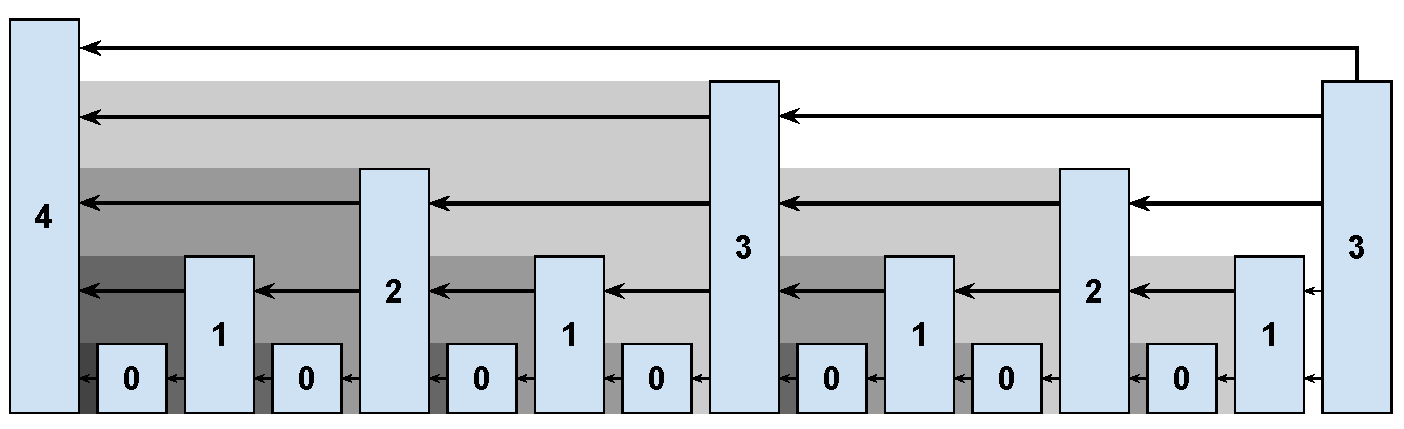
\includegraphics[width=0.9\columnwidth,keepaspectratio]{chapters/introduction/figures/level-shadows.pdf}
    \label{fig.hierarchy}
\end{figure}

\todo{applications to superlight wallets}
\todo{applications to sidechains}
\todo{applications to logspace mining}
\todo{the variable difficulty and $\Delta$-delay setting}
\todo{proofs of stake}

\ifdraft
\todo{Clean up paragraph}
In this section, we introduce the first
trustless construction for proof-of-work sidechains. We describe how to build
generic communication between blockchains. As one application, we give the
construction of a \emph{two-way pegged} asset which can be moved from one
blockchain to another while retaining its nature. We provide a high-level
construction in Solidity. Our construction works across a broad range of
blockchains requiring only two underlying properties. First, that the
\emph{source} blockchain is a proof-of-work blockchain supporting
Non-Interactive Proofs of Proof-of-Work (NIPoPoWs), a cryptographic primitive
which allows constructing succinct proofs \emph{about} events which occur in a
proof-of-work blockchain and which was recently introduced in~\cite{nipopows}.
Support for NIPoPoWs can be introduced to practically any
work-based cryptocurrency such as Bitcoin and Ethereum without a hard or soft
fork. Second, that the \emph{target} blockchain is able to validate such proofs
through smart contracts such as, e.g., Ethereum or Ethereum
Classic.
We give a formal proof of security of our construction via
reduction to NIPoPoW security under the assumption that the interoperating
blockchains are secure individually.
To our knowledge, we are the first to
provide such a construction in
full and prove its security.
\fi

\subsection{Summary of Contributions}
A summary of our contributions and their dependencies, with annotations
indicating where they are presented in this thesis, is visually illustrated in
Figure~\ref{fig.contributions}.

In summary, in this thesis we solve the problem of \emph{consensus compression}
for all decentralized blockchain consensus mechanisms. \textbf{For
proof-of-work}, we introduce the NIPoPoWs primitive (Chapter 3) and we give two
superblock-based constructions of succinct NIPoPoWs protocols in the Backbone
model: First the \emph{charity} construction (Chapter~\ref{chapter:work}), and
second the \emph{distill} construction (Chapter~\ref{chapter:variable}
and~\ref{chapter:superlight}). In the static synchronous model
(Chapter~\ref{chapter:work}), we prove our charity construction with
\emph{goodness} secure against $\frac{1}{2}$ adversaries, but succinct only in
the optimistic setting. Our charity construction \emph{without goodness} as well
as our distill construction are both secure and succinct against $\frac{1}{3}$
adversaries (Chapter~\ref{chapter:variable}). In the synchronous variable model
(Chapter~\ref{chapter:variable}), our distill construction is secure against a
$\frac{1}{3}$ adversary as long as difficulty is non-decreasing. Our charity
without goodness construction is secure against a $\frac{1}{3}$ adversary even
if difficult is not limited to non-decreasing. Both are succinct as long as
difficulty is not exponentially decreasing. Lastly, in the $\Delta$-bounded
delay setting (Chapter~\ref{chapter:variable}), both constructions are secure
and succinct under the same limitations, but only against a $\frac{1}{4}$
adversary. We give concrete parameter recommendations and run experiments and
simulations indicatively for the charity construction of
Chapter~\ref{chapter:work}. \textbf{For proof-of-stake}, we construct the ATMs
primitive and give signature-based construction (Chapter~\ref{chapter:stake}).
These are secure in the Ouroboros model, but offer only constant improvements
over full clients and hence do not achieve asymptotic succinctness.

We make use of these primitives to build \textbf{cross-chain transfer}
applications, which give rise to interoperability among blockchains, allowing
generic information transfer among work/work, work/stake, and stake/stake
chains. We give the definition of what constitutes a secure sidechain protocol
(Chapter~\ref{chapter:sidechains}) and put forth cross-chain protocols which we
prove secure. Our protocols can work natively or by leveraging smart contract
functionality. We show how they can be utilized to create one-way and two-way
pegs and discuss several deployment mechanisms which allow them to be deployed
as soft forks or better. Our protocols can also be used to build superlight
clients. Lastly, we show that our proof-of-work protocols specifically can be
utilized to build logarithmic-space miners (Chapter~\ref{chapter:superlight}),
providing exponential improvements over the state and communication complexity
of existing blockchain protocols.

\begin{figure}
    \caption{
      A roadmap of this thesis' structure.
      Our underlying model is shown above the double line.
      Our contributions are shown below the double line and comprise consensus
      compression primitives (above the dashed line) and their applications
      (below the dashed line). The respective chapters are indicated next to
      each topic.
    }
    \centering
    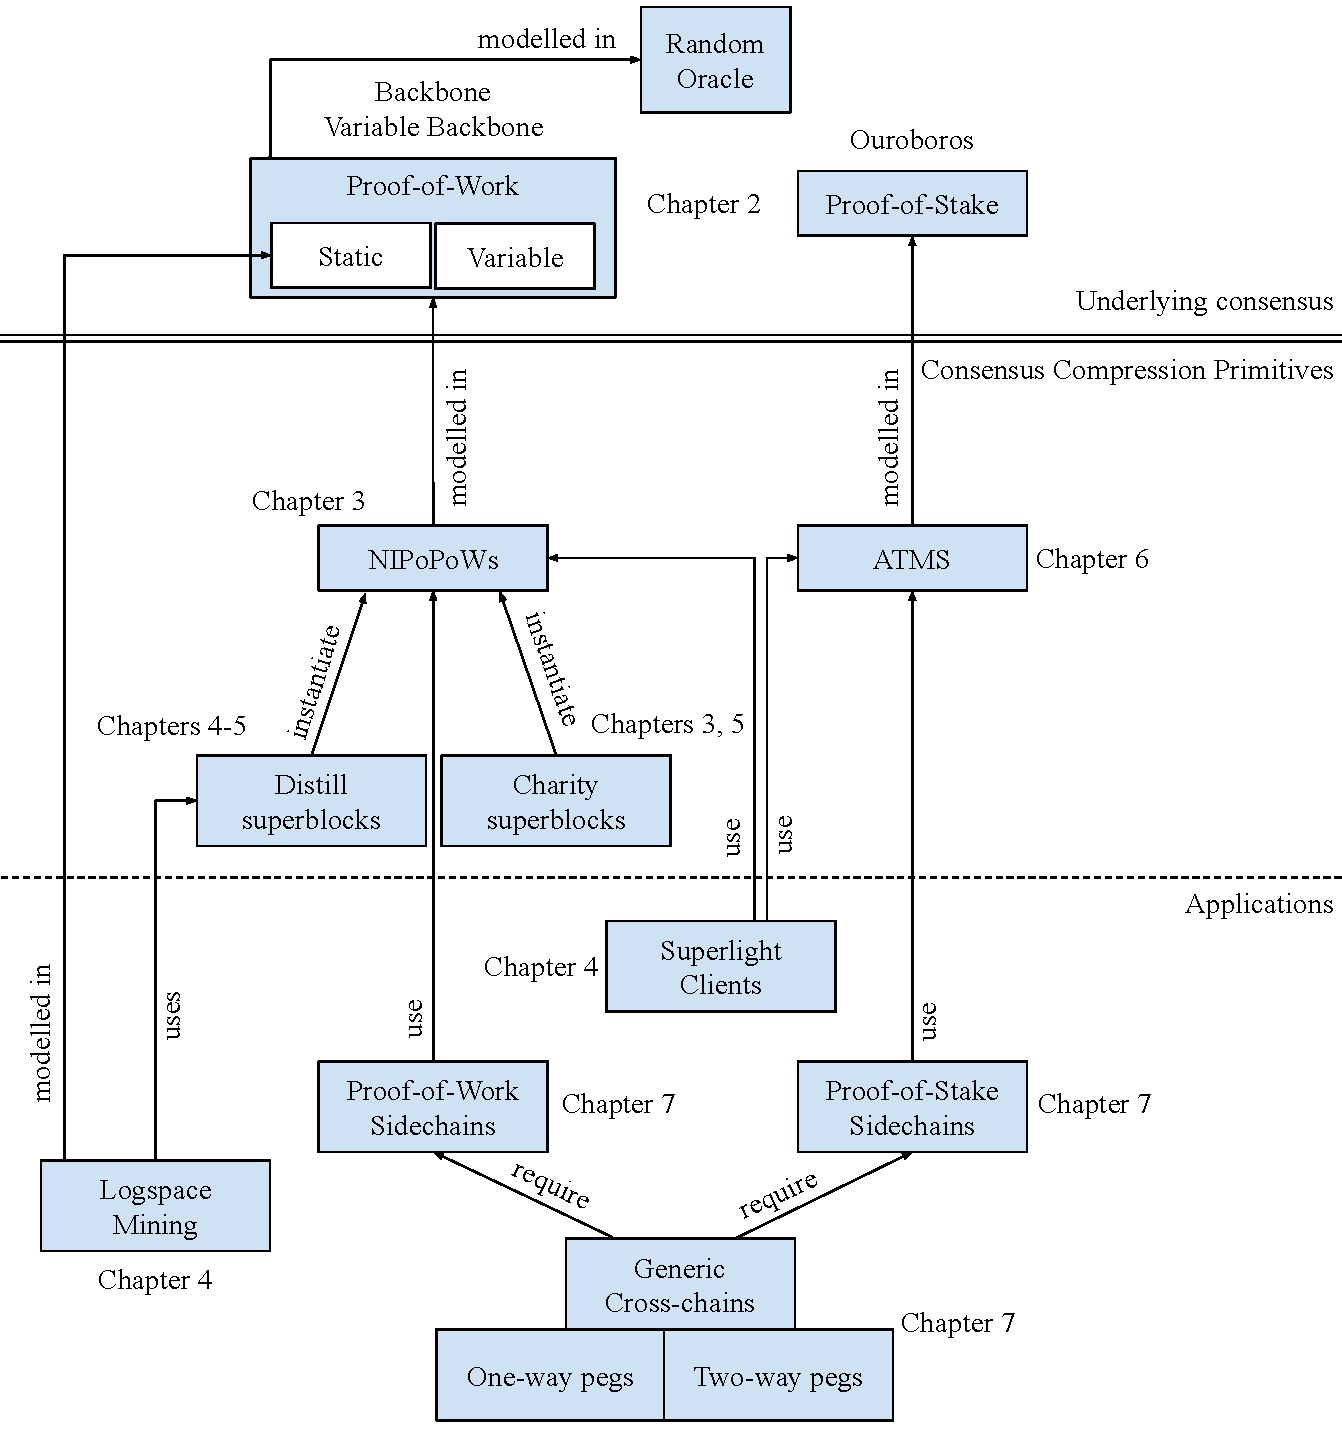
\includegraphics[width=\columnwidth,keepaspectratio]{chapters/introduction/figures/contributions.pdf}
    \label{fig.contributions}
\end{figure}
